\documentclass[a4paper, norsk, 10pt]{article}
%\usepackage[latin1]{inputenc}
\usepackage[utf8]{inputenc} 
\usepackage{multicol, fancyhdr}
\usepackage[norsk, english]{babel} % Tilpasning til norsk
\usepackage[margin=3cm]{geometry}
\usepackage{graphicx}
\usepackage{wrapfig}
%\usepackage{array, xcolor}
%\definecolor{ligttgray}{gray}{0.8}
\usepackage[mmddyyyy]{datetime}
\usepackage[table]{xcolor}
\usepackage{fancyhdr} %For å lage topptekst og bunntekst
\newcommand\tab[1][1cm]{\hspace*{#1}}
\pagestyle{fancy}
\fancyhead[R]{Øvingsoppgaver arrays, objects, skjemaer og animasjoner, mars 2018}

\title{\bfseries \huge Øvingsoppgaver skjemaer og animasjoner, mars 2018 \\ Informasjonsteknologi 2}
\date{}
\author{}

\begin{document}
\thispagestyle{fancy}
\maketitle

\section*{Om oppgavene}
Disse oppgavene er ment å jobbe med i de timene fremover hvor vi ikke er full klasse pga åpen dag og reiseuke. Dere velger det temaet der dere har mest behov for repetisjon dersom dere ikke rekker å gjøre alle oppgavene. \\
Skjemaoppgavene involverer også generell bearbeiding av DOM ved bruk av arrays/objects.\\
Oppgavene er hentet fra gamle eksamensoppgaver, og er en god repetisjon til heldagsprøven som kommer etter påske. Vi vil bruke disse oppgavene som grunnlag når vi jobber med løsningsstrategier og måloppnåelse i uke 12. \\

\section*{Oppgave 1: Skjema}
\textbf{Oppgaven er hentet fra eksamen vår 2015. Temaet er sykkelferier.}\\
\ \\
Du skal lage en applikasjon der brukeren skal kunne velge enten kort eller lang rute i «Østfold på hjul», velge attraksjoner og beregne pris. Kartet skal vises i applikasjonen.
Kort rute har en samlet overnattingspris på 3200 kr. Lang rute har en samlet overnattingspris på 7800 kr.\\
Når en bruker har valgt kort eller lang rute, skal det vises en liste med attraksjoner langs ruten: \\
\ \\
\begin{figure}[h!]
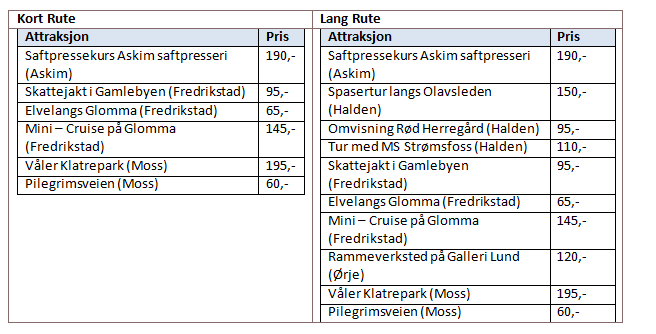
\includegraphics[width=12cm]{v15.png}
\end{figure}
\ \\
Fra lista som vises, skal brukeren kunne velge attraksjoner han/hun vil være med på, og samlet pris for turen skal skrives ut / vises.\\

\section*{Oppgave 2: Skjema}
\textbf{Oppgaven er hentet fra eksamen vår 2016. Temaet er reiser.} \\
\ \\
Du skal utvikle en enkel språktest for avisen. Brukerne skal kunne velge språket de ønsker å ta en test i, og applikasjonen skal da opprette spørsmål basert på dette valget.
Du trenger bare å lage en språktest for amerikansk under eksamen, men du skal gjøre det så enkelt som mulig å legge til andre språk og flere spørsmål i programkoden.\\
Brukerne skal få ett poeng for riktig svaralternativ og ett minuspoeng for feil svaralternativ i de forskjellige oppgavene. Hvis de får alt rett, skal de få en hyggelig melding om at de kan dette språket godt. Hvis de får mellom null og tre poeng, skal de få en melding om at avisen tilbyr språkkurs i New York. Får de mindre enn null poeng, skal de få en hyggelig melding som f.eks.: «Dette gikk ikke så bra, men det er håp for alle som vil lære et nytt språk!»\\
\ \\
Oppgave:\\
a) Lag applikasjonen.\\
b) Kommenter i koden, og redegjør for valgene du har gjort, i et eget dokument.\\
\ \\
Relevante spørsmål og lyd til oppgave 2 finner du i vedleggsfilene spraaktestsporsmaal.rtf og Oversetting.mp3.\\

\section*{Oppgave 3: Skjema}
\textbf{Oppgaven er hentet fra eksamen vår 2016. Temaet er reiser.} \\
\ \\
Du skal lage en applikasjon der man kan bestille språk- og kulturreiser til enten St. Petersburg, Amsterdam, New York eller Roma. På eksamensdagen skal alle byene være representert, men du skal kun gjøre løsningen for New York ferdig. Flere byer bør enkelt kunne legges til senere.\\
Det skal være mulig å velge\\
\begin{itemize} 
\item destinasjon (by)
\item reiseperiode (sommer- eller vinterhalvår)
\item antall dobbeltrom
\item antall enkeltrom
\item hotell
\item kulturpass for kulturelle aktiviteter (pris kr 700)
\end{itemize} 
\ \\
I vedleggsfilen hoteller.rtf er det en oversikt over hotellene som avisen samarbeider med, og som brukerne skal kunne velge blant. Til eksamen behøver du bare å bruke fem av hotellene, men programkoden bør enkelt kunne utvides til å legge inn alle hotellene.\\
\ \\
Brukerne skal kunne se valg de har gjort underveis i bestillingen, og når som helst i bestillingsrutinen se prisen på de valgene de har gjort.\\
\ \\
Oppgave \\
a) Lag applikasjonen.\\
b) Kommenter i koden, og redegjør for valgene du har gjort, i et eget dokument.\\

\section*{Oppgave 4: Skjema}
\textbf{Oppgaven er hentet fra eksamen høst 2016. Temaet er matkasser.}\\
\ \\
Bestillingen av matkassene skal foregå på nettsiden. Du skal lage en applikasjon der kunden (brukeren) kan velge en matkasse som inneholder to eller tre middager, og hvor mange personer middagene skal lages til.\\
\ \\
Når brukeren har valgt matkasse, skal det komme opp et bilde som illustrerer om det er to eller tre middager som er valgt. Applikasjonen bør sjekke om antall personer som er registrert, er innenfor lovlige/sannsynlige verdier.\\
Prisen beregnes ut fra valgene, og du kan regne med 80 kroner per person per måltid. Bestilles det matkasser til fem personer eller mer, vil prisen per person være 70 kroner.\\
Applikasjonen skal bekrefte valgene som er gjort, og navnet og adressen til den som bestiller, skal legges inn og vises sammen med de andre opplysningene.\\
\ \\
(Bestillingen vil på en virkelig nettside måtte sendes/lagres ved hjelp av for eksempel e-post eller en fil, men på eksamen trenger du ikke gjøre noe med dette.)\\

\section*{Oppgave 5: Skjema}
\textbf{Oppgaven er hentet fra eksamen høst 2016. Temaet er matkasser.}\\
\ \\
Fiskerne som leverer til Fra fjord til bord, har sine spesialiteter: hvit fisk og skalldyr fra fjorden og laks fra Mandalselva. Det lages en bestillingsliste hver uke, slik at fiskerne kan beregne hvor mye de skal hente opp fra havet.\\
Under ser du et utdrag av råvaretabellen til Fra fjord til bord. Tabellen forteller hvor mange gram av hvert slag de mener må beregnes per person fra bestillingsprogrammet.\\
\ \\
\textbf{Råvaretabell:}\\
\ \\
\begin{tabular}{ c | c | c | c | c | c | c }
& \textbf{Torsk} & \textbf{Sei} & \textbf{Makrell} & \textbf{Reker} & \textbf{Krabbe} & \textbf{Laks} \\
\hline
Barn & 200 & 200 & 200 & 250 & 300 & 200 \\
Ungdom & 300 & 300 & 300 & 500 & 500 & 300 \\
Voksne & 350 & 350 & 350 & 500 & 600 & 350 \\
\end{tabular}
\ \\
\ \\
Middagene for uke 26 i 2016 ser slik ut:\\
Middag 1: Sørlandsk krabbesuppe \\
Middag 2: Mandalstorsk i smørsaus med Holumspoteter \\
Middag 3: Laks fra Laudal i spinat (bare for dem som har bestilt tre middager)\\
Fra fjord til bord får bestillingene på e-post. De må registrere bestillingene i en slik tabell:\\
\ \\
\begin{tabular}{ c | c | c | c | c  }
\textbf{Uke nr.} & \textbf{Antall middager} &  \textbf{Barn} &  \textbf{Ungdom} &  \textbf{Voksne} \\
\hline
26 & 2 & 1 & 1 & 2\\
26 & 3 & 0 & 2 & 2 \\
26 & 2 & 0 & 0 & 1 \\
26 & 3 & 0 & 0 & 2 \\
26 & 2 & 3 & 0 & 3 \\
27 & 2 & 1 & 1 & 2 \\
27 & 2 & 1 & 1 & 2 \\
\end{tabular}
 \ \\
 \clearpage
\noindent Med utgangspunkt i informasjonen over blir du bedt om å utføre følgende oppgaver:\\
a) Lag en rutine for å registrere bestillingene i bestillingstabellen. Bestillingene skal vises på skjermen. (Grønnsaker som hører til bestillingen, beregnes av samarbeidende bønder og gartnere, så dette behøver du ikke ta hensyn til.)\\
b) Lag en rutine som beregner totalbehovet for hvert fiskeslag i uke 26. Skriv først en pseudokode eller lag et flytdiagram for rutinen, og programmer deretter løsningen.\\

\section*{Oppgave 6: Animasjoner}
\textbf{Oppgaven er hentet fra eksamen vår 2014. Temaet er trafikksikkerhet.}\\
\ \\
Du skal lage en applikasjon som skal brukes i en holdningskampanje for å senke farten på kjøretøy. Applikasjonen skal vise et bilde av en bil på en vei med 60-sone.\\ Brukeren skal kunne taste inn farten til en bil. Dersom farten til bilen er over 60 km/t, skal det kjøres en lydfil som ender i et bilkrasj. Om farten er under 60 km/t, skal det avspilles en lydfil med en bil som kjører, kombinert med fuglekvitter. Applikasjonen skal så gå over i en oppfordrende tekst: "Senk farten!"\\
\ \\
Vedlagt finnes foto av en vei og en bil. I tillegg finner du lydfiler som du skal redigere til to ulike filer: én som skal brukes om farten er over 60 km/t, og én som skal brukes om farten er under 60 km/t.\\

\section*{Oppgave 7: Animasjoner}
\textbf{Oppgaven er hentet fra eksamen vår 2015. Temaet er sykkelferier.}\\
\ \\
Du skal utvikle en applikasjon med utgangspunkt i det vedlagte kartet over sykkelrutene. Fylkeskommunen ønsker videopresentasjoner av fem steder langs sykkelrutene på kartet: Askim, Ørje, Halden, Fredrikstad og Moss.\\
\ \\
Under eksamen er det nok at du legger inn videopresentasjoner for to av stedene: Halden og Fredrikstad. For Fredrikstad skal du bruke den vedlagte videofila uten å redigere den. For Halden skal du bruke de vedlagte fotoene og videoen og sette dem sammen til en videopresentasjon på en lengde på mellom 1 og 1,5 minutt.\\
Når brukere klikker i kartet på henholdsvis Halden eller Fredrikstad, skal det åpnes et nytt vindu der videopresentasjonen skal kjøres. Presentasjonene av stedene må kunne kjøres så mange ganger som det er ønskelig, og i den rekkefølgen brukeren velger\\

\section*{Oppgave 8: Animasjoner}
\textbf{Oppgaven er hentet fra eksamen vår 2016. Temaet er reiser.} 	\\
\ \\
En regionavis ønsker å etablere en reiseklubb for abonnentene sine med språk- og kulturopplevelser som tema. De ønsker derfor å utvikle interaktive applikasjoner til nettsiden sin for å skape oppmerksomhet rundt og markedsføre reiseklubben.\\
\ \\
Avisen ønsker seg en nettbasert løsning som tar utgangspunkt i tre bilder av byene St. Petersburg, New York og Roma. Du skal lage ett bilde med maksimum bredde på 750 piksler og valgfri høyde med de tre bildene. Brukeren skal kunne velge hvert av bildene med f.eks. en klikkhendelse, og da skal følgende valg være mulig:\\
\begin{itemize} 
\item Bilde nummer 1 (St. Petersburg) skal vises i full størrelse.
\item Bilde nummer 2 (Roma) skal spille av den vedlagte videoen. I den skal du først klippe bort de tolv første sekundene.
\item Bilde nummer 3 (New York) skal ta brukeren til en applikasjon der han skal tippe hvilken bygning som er på bildet. Hvis han svarer rett, skal han få en hyggelig melding, f.eks.: «Du vet allerede noe om New York – hva med å lære mer?» Hvis han svarer galt, kan teksten «Det var ikke rett – kanskje på tide med en New York-tur?» komme opp.
\end{itemize}
Bilder og video til oppgaven finner du i vedleggsfilen.

\section*{Oppgave 9: Animasjoner}
\textbf{Oppgaven er hentet fra eksamen vår 2017. Temaet er fornybar energi.}\\
\ \\
Det har blitt stadig mer populært med fornybare energikilder til bruk i private hjem og fritidseiendommer. Mange ønsker f.eks. å finne ut hvor mye energi de kan produsere med ulike former for fornybare energikilder, eller se på hvordan fornybare energikilder virker/fungerer.\\
\ \\
Du skal lage en applikasjon som viser en vindmølle plassert i et landskap. I applikasjonen skal bladene på vindmølla kunne roteres, og det skal være elementer i landskapet som skal animeres når vindstyrken endres.\\
I applikasjonen skal brukeren kunne oppgi betegnelsen på en vindstyrke, og applikasjonen skal kunne vise virkningene i landskapet for den vindstyrken. Du finner en oversikt i vedlegget over ulike vindstyrker og beskrivelser av virkninger av vinden i landskapet. På eksamen er det nok at du lager animasjoner for vindstyrkene stille, lett bris og stiv kuling. Bladene på vindmølla skal ha ulik fart i de tre tilfellene, og når en vindstyrke er valgt, skal den også vises på skjermen («0–0.2 m/s», «3.4–5.4 m/s» eller «13.9–17.1 m/s»). Lyden av vind skal spilles når lett bris eller stiv kuling blir valgt. En fil med vindlyd ligger vedlagt. Det skal være mulig å kjøre animasjonene flere ganger og i den rekkefølgen brukeren ønsker.\\
\ \\
Du kan tegne eller lage et bilde ved å kombinere elementer fra vedlagte foto/skisser, f.eks. lik tegningen under. Du kan også utforme bildet helt annerledes om du ønsker det.\\
\begin{figure}[h!]
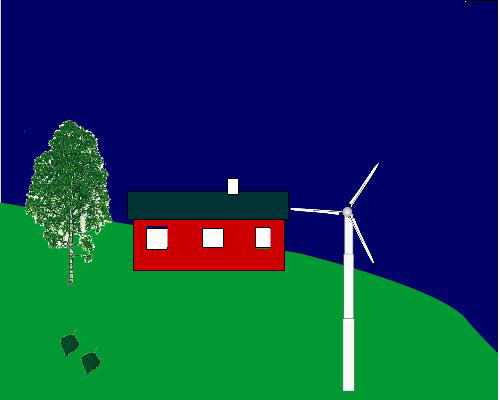
\includegraphics[width=10cm]{v17.png}
\end{figure}

\end{document}